% Options for packages loaded elsewhere
\PassOptionsToPackage{unicode}{hyperref}
\PassOptionsToPackage{hyphens}{url}
\PassOptionsToPackage{dvipsnames,svgnames*,x11names*}{xcolor}
%
\documentclass[
  11pt,
  ignorenonframetext,
  aspectratio=169,
  aspectratio=169]{beamer}
\usepackage{pgfpages}
\setbeamertemplate{caption}[numbered]
\setbeamertemplate{caption label separator}{: }
\setbeamercolor{caption name}{fg=normal text.fg}
\beamertemplatenavigationsymbolsempty

%%
%%% Definition of colors
%%% Source: https://latexcolor.com/
\definecolor{blanchedalmond}{rgb}{1.0, 0.92, 0.8}
\definecolor{blond}{rgb}{0.98, 0.94, 0.75}
%%% End of definition of colors
%%

% Prevent slide breaks in the middle of a paragraph
\widowpenalties 1 10000
\raggedbottom
\usepackage{lmodern}
\usepackage{amssymb,amsmath}
\usepackage{soul}
\usepackage{ifxetex,ifluatex}
\ifnum 0\ifxetex 1\fi\ifluatex 1\fi=0 % if pdftex
  \usepackage[T1]{fontenc}
  \usepackage[utf8]{inputenc}
  \usepackage{textcomp} % provide euro and other symbols
\else % if luatex or xetex
  \usepackage{unicode-math}
  \defaultfontfeatures{Scale=MatchLowercase}
  \defaultfontfeatures[\rmfamily]{Ligatures=TeX,Scale=1}
  \setmainfont[]{Hack Nerd Font}
\fi
\usetheme[]{Frankfurt}
\usecolortheme{beaver}
\usefonttheme{professionalfonts}
\usefonttheme{serif} % use mainfont rather than sansfont for slide text
% Use upquote if available, for straight quotes in verbatim environments
\IfFileExists{upquote.sty}{\usepackage{upquote}}{}
\IfFileExists{microtype.sty}{% use microtype if available
  \usepackage[]{microtype}
  \UseMicrotypeSet[protrusion]{basicmath} % disable protrusion for tt fonts
}{}
\makeatletter
\@ifundefined{KOMAClassName}{% if non-KOMA class
  \IfFileExists{parskip.sty}{%
    \usepackage{parskip}
  }{% else
    \setlength{\parindent}{0pt}
    \setlength{\parskip}{6pt plus 2pt minus 1pt}}
}{% if KOMA class
  \KOMAoptions{parskip=half}}
\makeatother
\usepackage{xcolor}
\IfFileExists{xurl.sty}{\usepackage{xurl}}{} % add URL line breaks if available
\IfFileExists{bookmark.sty}{\usepackage{bookmark}}{\usepackage{hyperref}}
\hypersetup{
  pdftitle={My wonderful presentation},
  pdfauthor={Alexey Gumirov},
  colorlinks=true,
  linkcolor=Maroon,
  filecolor=Maroon,
  citecolor=Blue,
  urlcolor=red,
  pdfcreator={LaTeX via pandoc}}
\urlstyle{same} % disable monospaced font for URLs
\newif\ifbibliography
\usepackage{listings}
\newcommand{\passthrough}[1]{#1}
\lstset{defaultdialect=sh}
\lstset{framexleftmargin=0mm, frame=trBL,backgroundcolor=\color{blanchedalmond!5},numbers=left,numberstyle=\scriptsize,basicstyle=\small}
\lstset{aboveskip=5mm,belowskip=5mm,xleftmargin=20pt,xrightmargin=5pt}
% \lstset{prebreak={\raisebox{0ex}[0ex][0ex]}}
% \lstset{postbreak={\raisebox{0ex}[0ex][0ex]\space}}
\lstset{breaklines=true,breakatwhitespace=true}
\usepackage{longtable,booktabs}
\usepackage{caption}
% Make caption package work with longtable
\makeatletter
\def\fnum@table{\tablename~\thetable}
\makeatother
\usepackage{graphicx,grffile}
\makeatletter
\def\maxwidth{\ifdim\Gin@nat@width>\linewidth\linewidth\else\Gin@nat@width\fi}
\def\maxheight{\ifdim\Gin@nat@height>\textheight\textheight\else\Gin@nat@height\fi}
\makeatother
% Scale images if necessary, so that they will not overflow the page
% margins by default, and it is still possible to overwrite the defaults
% using explicit options in \includegraphics[width, height, ...]{}
\setkeys{Gin}{width=\maxwidth,height=\maxheight,keepaspectratio}
% Set default figure placement to htbp
\makeatletter
\def\fps@figure{htbp}
\makeatother
\usepackage[normalem]{ulem}
% Avoid problems with \sout in headers with hyperref
\pdfstringdefDisableCommands{\renewcommand{\sout}{}}
\setlength{\emergencystretch}{3em} % prevent overfull lines
\providecommand{\tightlist}{%
  \setlength{\itemsep}{0pt}\setlength{\parskip}{0pt}}
\setcounter{secnumdepth}{-\maxdimen} % remove section numbering

%
% When using babel or polyglossia with biblatex, loading csquotes is recommended 
% to ensure that quoted texts are typeset according to the rules of your main language.
%
\usepackage{csquotes}

%
% blockquote
%
\definecolor{blockquote-border}{RGB}{221,221,221}
\definecolor{blockquote-text}{RGB}{89,89,89}
\usepackage{mdframed}
\newmdenv[rightline=false,bottomline=false,topline=false,linewidth=3pt,linecolor=blockquote-border,skipabove=\parskip]{customblockquote}
\renewenvironment{quote}{\begin{customblockquote}\list{}{\rightmargin=0em\leftmargin=0em}%
\item\relax\color{blockquote-text}\ignorespaces}{\unskip\unskip\endlist\end{customblockquote}}

%
% Source Sans Pro as the de­fault font fam­ily
% Source Code Pro for monospace text
%
% 'default' option sets the default 
% font family to Source Sans Pro, not \sfdefault.
%


\title{My wonderful presentation}
\author{Alexey Gumirov}
\date{17 Fevereiro 2023}
\institute{My home office}
\titlegraphic{
\includegraphics{img/aleph0.png}}
\logo{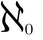
\includegraphics{img/aleph0-small.png}}

\begin{document}
\frame{\titlepage}

\begin{frame}
  \tableofcontents[hideallsubsections]
\end{frame}
\hypertarget{general-information}{%
\section{General information}\label{general-information}}

\begin{frame}{Themes, fonts, etc.}
\protect\hypertarget{themes-fonts-etc.}{}
\begin{itemize}
\tightlist
\item
  I use default \textbf{pandoc} themes.
\item
  This presentation is made with \textbf{Frankfurt} theme and
  \textbf{beaver} color theme.
\item
  I like \textbf{professionalfonts} font scheme.
\end{itemize}
\end{frame}

\begin{frame}{Links}
\protect\hypertarget{links}{}
\begin{itemize}
\tightlist
\item
  Matrix of beamer themes:
  \url{https://hartwork.org/beamer-theme-matrix/}
\item
  Font themes:
  \href{http://www.deic.uab.es/~iblanes/beamer_gallery/index_by_font.html}{http://www.deic.uab.es/\textasciitilde iblanes/beamer\emph{gallery/index}by\_font.html}
\item
  Nerd Fonts: \url{https://nerdfonts.com}
\end{itemize}
\end{frame}

\hypertarget{formatting}{%
\section{Formatting}\label{formatting}}

\begin{frame}{Text formatting}
\protect\hypertarget{text-formatting}{}
Normal text. \emph{Italic text} and \textbf{bold text}. \st{Strike out}
is supported.
\end{frame}

\begin{frame}{Fórmulas}
\protect\hypertarget{fuxf3rmulas}{}
\begin{itemize}
\tightlist
\item
  A energia cinética é dada por \$\$ K = \textbackslash frac\{1\}\{2\}
  mv\^{}2 \$\$.
\item
  A energia cinética é dada por \$ K = \textbackslash frac\{1\}\{2\}
  mv\^{}2 \$.
\item
  A energia cinética é dada por \$\$K = \textbackslash frac\{1\}\{2\}
  mv\^{}2\$\$.
\item
  A energia cinética é dada por \$K = \textbackslash frac\{1\}\{2\}
  mv\^{}2\$.
\end{itemize}
\end{frame}

\begin{frame}{Notes}
\protect\hypertarget{notes}{}
\begin{quote}
This is a note.

\begin{quote}
Nested notes are not supported. And it continues.
\end{quote}
\end{quote}
\end{frame}

\begin{frame}{Blocks}
\protect\hypertarget{blocks}{}
\begin{block}{This is a block A}
\protect\hypertarget{this-is-a-block-a}{}
\begin{itemize}
\tightlist
\item
  Line A
\item
  Line B
\end{itemize}
\end{block}

\begin{block}{}
\protect\hypertarget{section}{}
New block without header.
\end{block}

\begin{block}{This is a block B.}
\protect\hypertarget{this-is-a-block-b.}{}
\begin{itemize}
\tightlist
\item
  Line C
\item
  Line D
\end{itemize}
\end{block}
\end{frame}

\begin{frame}[fragile]{Listings}
\protect\hypertarget{listings}{}
Listings out of the block.

\begin{lstlisting}[language=sh]
#!/bin/bash
echo "Hello world!"
echo "line"
\end{lstlisting}

\begin{block}{Listings in the block.}
\protect\hypertarget{listings-in-the-block.}{}
\begin{lstlisting}[language=sh]
#!/bin/bash
echo "Hello world!"
echo "line"
\end{lstlisting}
\end{block}
\end{frame}

\begin{frame}{Table}
\protect\hypertarget{table}{}
\begin{longtable}[]{@{}lrc@{}}
\toprule\noalign{}
\textbf{Item} & \textbf{Description} & \textbf{Q-ty} \\
\midrule\noalign{}
\endhead
\bottomrule\noalign{}
\endlastfoot
Item A & Item A description & 2 \\
Item B & Item B description & 5 \\
Item C & N/A & 100 \\
\end{longtable}
\end{frame}

\begin{frame}[fragile]{Single picture}
\protect\hypertarget{single-picture}{}
This is how we insert picture. Caption is produced automatically from
the alt text.

\begin{lstlisting}
![Aleph 0](img/aleph0.png) 
\end{lstlisting}

\begin{figure}
\centering

\includegraphics{img/aleph0.png}
\caption{Aleph 0}
\end{figure}
\end{frame}

\begin{frame}[fragile]{Two or more pictures in a raw}
\protect\hypertarget{two-or-more-pictures-in-a-raw}{}
Here are two pictures in the raw. We can also change two pictures size
(height or width).

\begin{block}{}
\protect\hypertarget{section-1}{}
\begin{lstlisting}
![](img/aleph0.png){height=10%}\ ![](img/aleph0.png){height=30%} 
\end{lstlisting}


\includegraphics[width=\textwidth,height=0.1\textheight]{img/aleph0.png}~
\includegraphics[width=\textwidth,height=0.3\textheight]{img/aleph0.png}
\end{block}
\end{frame}

\begin{frame}{Lists}
\protect\hypertarget{lists}{}
\begin{enumerate}
\tightlist
\item
  Idea 1
\item
  Idea 2

  \begin{itemize}
  \tightlist
  \item
    genius idea A
  \item
    more genius 2
  \end{itemize}
\item
  Conclusion
\end{enumerate}
\end{frame}

\begin{frame}{Two columns of equal width}
\protect\hypertarget{two-columns-of-equal-width}{}
\begin{columns}[T]
\begin{column}{0.48\textwidth}
Left column text.

Another text line.
\end{column}

\begin{column}{0.48\textwidth}
\begin{itemize}
\tightlist
\item
  Item 1.
\item
  Item 2.
\item
  Item 3.
\end{itemize}
\end{column}
\end{columns}
\end{frame}

\begin{frame}{Two columns of with 40:60 split}
\protect\hypertarget{two-columns-of-with-4060-split}{}
\begin{columns}[T]
\begin{column}{0.4\textwidth}
Left column text.

Another text line.
\end{column}

\begin{column}{0.6\textwidth}
\begin{itemize}
\tightlist
\item
  Item 1.
\item
  Item 2.
\item
  Item 3.
\end{itemize}
\end{column}
\end{columns}
\end{frame}

\begin{frame}{Three columns with equal split}
\protect\hypertarget{three-columns-with-equal-split}{}
\begin{columns}[T]
\begin{column}{0.48\textwidth}
Left column text.

Another text line.
\end{column}

\begin{column}{0.48\textwidth}
Middle column list:

\begin{enumerate}
\tightlist
\item
  Item 1.
\item
  Item 2.
\end{enumerate}
\end{column}

\begin{column}{0.48\textwidth}
Right column list:

\begin{itemize}
\tightlist
\item
  Item 1.
\item
  Item 2.
\end{itemize}
\end{column}
\end{columns}
\end{frame}

\begin{frame}{Three columns with 30:40:30 split}
\protect\hypertarget{three-columns-with-304030-split}{}
\begin{columns}[T]
\begin{column}{0.3\textwidth}
Left column text.

Another text line.
\end{column}

\begin{column}{0.4\textwidth}
Middle column list:

\begin{enumerate}
\tightlist
\item
  Item 1.
\item
  Item 2.
\end{enumerate}
\end{column}

\begin{column}{0.3\textwidth}
Right column list:

\begin{itemize}
\tightlist
\item
  Item 1.
\item
  Item 2.
\end{itemize}
\end{column}
\end{columns}
\end{frame}

\begin{frame}{Two columns: image and text}
\protect\hypertarget{two-columns-image-and-text}{}
\begin{columns}[T]
\begin{column}{0.48\textwidth}

\includegraphics[width=\textwidth,height=0.5\textheight]{img/aleph0.png}
\end{column}

\begin{column}{0.48\textwidth}
Text in the right column.

List from the right column:

\begin{itemize}
\tightlist
\item
  Item 1.
\item
  Item 2.
\end{itemize}
\end{column}
\end{columns}
\end{frame}

\begin{frame}{Two columns: image and table}
\protect\hypertarget{two-columns-image-and-table}{}
\begin{columns}[T]
\begin{column}{0.48\textwidth}

\includegraphics[width=\textwidth,height=0.5\textheight]{img/aleph0.png}
\end{column}

\begin{column}{0.48\textwidth}
\begin{longtable}[]{@{}lc@{}}
\toprule\noalign{}
\textbf{Item} & \textbf{Option} \\
\midrule\noalign{}
\endhead
\bottomrule\noalign{}
\endlastfoot
Item 1 & Option 1 \\
Item 2 & Option 2 \\
\end{longtable}
\end{column}
\end{columns}
\end{frame}

\begin{frame}{Fancy layout}
\protect\hypertarget{fancy-layout}{}
\begin{block}{Proposal}
\protect\hypertarget{proposal}{}
\begin{itemize}
\tightlist
\item
  Point A
\item
  Point B
\end{itemize}
\end{block}

\begin{columns}[T]
\begin{column}{0.48\textwidth}
\begin{block}{Pros}
\protect\hypertarget{pros}{}
\begin{itemize}
\tightlist
\item
  Good
\item
  Better
\item
  Best
\end{itemize}
\end{block}
\end{column}

\begin{column}{0.48\textwidth}
\begin{block}{Cons}
\protect\hypertarget{cons}{}
\begin{itemize}
\tightlist
\item
  Bad
\item
  Worse
\item
  Worst
\end{itemize}
\end{block}
\end{column}
\end{columns}

\begin{block}{Conclusion}
\protect\hypertarget{conclusion}{}
\begin{itemize}
\tightlist
\item
  Let's go for it!
\item
  No way we go for it!
\end{itemize}
\end{block}
\end{frame}

\end{document}
